\documentclass[12pt]{scrartcl}

 

\usepackage[utf8]{inputenc}

\usepackage[T1]{fontenc}

\usepackage{lmodern}

\usepackage[ngerman]{babel}

\usepackage{amsmath}

\usepackage{graphicx}


 

\title{Versuch E2\\ Der Halleffekt}

\author{Frederik Strothmann, Henrik Jürgens}

\date{\today}


\begin{document}


 %deckblatt erstellen

\maketitle
\tableofcontents
\newpage

%einleitung zu dem experiment

\section{Einleitung}

In diesem Versuch soll das Magnetfeld einer kurzen Spule auf ihrer Mittelachse ausmessen und dabei einfache elektrische Grundschaltungen angewendet werden. Zur Messung benutzen wir eine Hallsonde, die zu diesem Zweck vorher geeicht werden muß. Die Hallsonde liefert eine Spannung, die proportional zum Magnetfeld ist, aber schwierig zu messen ist, da sie im Millivoltbereich liegt und einige Hallsondentypen eine hohen Innenwiderstand haben. Die Ausgangsspannung der Hallsonde wird daher in diesem Versuch mit einer Kompensationsschaltung bestimmt. Den Widerstand der Hallsonde messen Sie mit der
Wheatstoneschen Brückenschaltung.

%versuchsaufbau mit skizze

\section{Versuchsaufbau}
Der Versuchsaufbau besteht haupsächlich aus zwei Komponenten, der Spule mit der Hallsonde und dem Steuerkasten.
Der Schaltplan ist in Abbilung \ref{fig:aufbau} zu sehen.

\begin{figure}[htbp] 
  \centering
    \includegraphics[scale = 0.5]{kasten_und_spule.JPG}
  	\caption[Foto der beiden Hauptbestandteile des Versuchs]{Foto der beiden Hauptbestandteile des Versuchs\footnotemark}
  \label{fig:kasten_und_spule}
\end{figure}
\footnotetext{Graphik wurde am 19.08.2014 von der Seite: http://www.atlas.uni-wuppertal.de/~kind/apjpg/ap1e2a.JPG entnommen}

\begin{figure}[htbp] 
  \centering
    \includegraphics[scale = 0.5]{kasten.JPG}
  	\caption[Foto des Schaltkastens]{Foto des Schaltkastens\footnotemark}
  \label{fig:kasten}
\end{figure}
\footnotetext{Graphik wurde am 19.08.2014 von der Seite: http://www.atlas.uni-wuppertal.de/~kind/apjpg/ap1e2vkg.JPG entnommen}

\section{Versuchsdurchführung}


\subsection{Praktische Durchführung}

\begin{enumerate}
\item Schaltskizze \newline

\begin{figure}[htbp] 
	  \centering
	    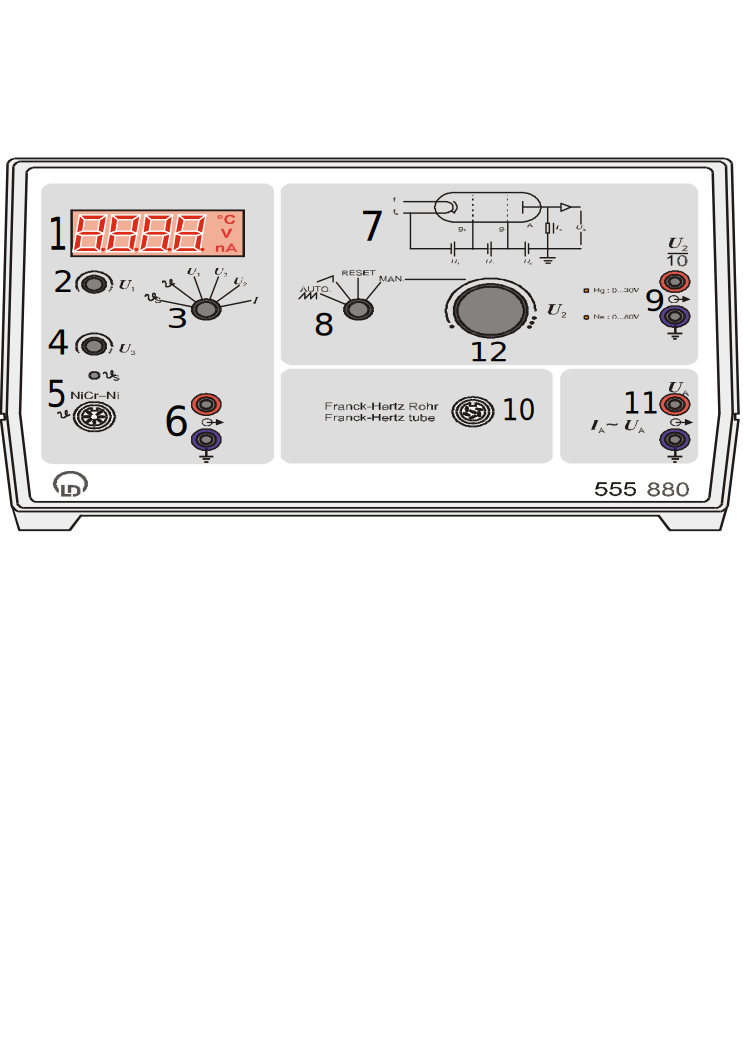
\includegraphics[trim = 1mm 135mm 1mm 30mm, clip, scale = 1]{aufbau.pdf}
	  	\caption[Schaltskizze des Versuchsaufbaus]{Schaltskizze des Versuchsaufbaus\footnotemark}
	  \label{fig:aufbau}
	\end{figure}
	\footnotetext{Abbildung entnommen von http://www.atlas.uni-wuppertal.de/~kind/E2.pdf Seite 7 am 19.08.2014}

\begin{itemize}
\item 1,5V: Batterie

\item S: Schalter für die Batterie

\item P$_\text{M}$: Potentiometer zum Einstellen der maximalen Kompensationsspannung

\item R$_\text{M}$: Wiederstand für die Strombegrenzung von P$_\text{M}$ und der Batterie

\item U$_\text{KM}$: Bananenbuchse, zum messen der Kompensationsspannung

\item P$_\text{K}$: Präzisionspotentiometer mit Skala

\item A: Abgriff am Potentiometer P$_\text{K}$, der das Potentiometer an die Widerstände R$_\text{1}$ und $_\text{2}$ aufteilt

\item I$_\text{0}$: Nullpunktgalvanometer. Mit Taster zum erhöhen der Empfindlichkeit um den Faktor 10. S schaltet den Messverstärker ein.

\item B$_\text{UH}$: Anschlüsse für die Hallsondenspannung

\item R$_\text{0}$: Bekannter Widerstand

\item S$_\text{R}$: Schalter um den Widerstand R$_\text{0}$ in den Stromkreis einzufügen und die Wheatstonesche Brücke zu vervollständigen

\item 12V: Buchsen für Spannungsquelle des Hallstroms

\item P$_\text{H}$: Potentiometer zum einstellen des Hallstroms

\item R$_\text{H}$: Vorwiderstand zur Begrenzung des Hallstroms

\item I$_\text{H}$: Drehspulamperemeter zur Messung des maximalen Hallstroms

\item B$_\text{IH}$: Anschlüsse für den Hallstrom

\end{itemize}

\item Vorversuche: \newline
a) Schließen Sie die Spule an das Netzgerät an und stellen Sie einen Strom von 1A ein. Achten Sie auf die richtige Polarität des Magnetfeldes, damit es keine negativen Hallspannungen gibt (siehe b)).
\newline
b) Schließen Sie an die Buchsen mit der Bezeichnung 12 Volt für I-Hall des Versuchskästchens die 12–Volt–Festspannungsquelle an. Achten Sie auf die angegebene Polarität (+ und –). Die Hallsonde kann zwar mit beliebiger Stromrichtung arbeiten. In Ihrem Versuchskästchen befindet sich aber ein weiteres Drehspulamperemeter für den Hallstrom, das keine negativen Ströme anzeigen kann. Außerdem würden Sie negative Hallspannungen bekommen, die
Sie mit der gegebenen Schaltung nicht kompensieren können. Stellen Sie den
maximalen Hallstrom ein (siehe Angabe auf Ihrem Versuchsaufbau! Je nach
Sondentyp liegt der maximale Hallstrom zwischen 5 und 100 mA. Der Vorwiderstand
R$_H$ im Versuchskästchen begrenzt den Hallstrom auf zulässige Werte).
\newline
c) Schieben Sie die Hallsonde in die Mitte der Spule. Stellen Sie dann eine maximale Kompensationsspannung so ein, daß bei dieser Anordnung die Hallspannung noch kompensiert werden kann und gleichzeitig eine leichte Umrechnung von Skalenteilen auf die Kompensationsspannung (zwischen Punkt A und dem unteren Punkt U$_{KM}$) möglich ist. Die Potentiometerskala zeigt Ihnen das Verhältnis von R$_2$ zu R$_1$ + R$_2$.
”0“ bedeutet R$_2$ = 0$\Omega$,”10“ (oder
0,00 hinter 9,99) bedeutet R$_1$ = 0$\Omega$. Da sich die Spannung der Batterie im Laufe der Zeit verändern kann, sollten Sie U$_{KM}$ öfter überprüfen und gegebenenfalls korrigieren
\item Eichung der Hallsonde 
\newline
a) Bestimmen Sie den Ort der Hallsonde in der Spule, an dem die Hallspannung maximal ist. In diesem Punkt können Sie annehmen, daß eine unendlich lange
Spule vorliegt. (Schätzen Sie die Winkel
$\theta_1$ und $\theta_2$ aus 
\begin{align}
B_z = \frac{1}{2} \mu_0 I_S N (\cos(\theta_1) - \cos(\theta_2)) 
\end{align}

 ab und vergleichen Sie den gemessenen Wert des Magnetfeldes mit dem Wert nach
 \begin{align}
 B_Z = \mu_0 I_S N
\end{align}
 Für N können Sie einen Wert von 13000/m annehmen; die Spule hat 10 Lagen mit etwa 1300 Windungen pro Meter).
\newline
b) Messen Sie dort die Abhängigkeit der Hallspannung vom Magnetfeld, indem
Sie den Spulenstrom variieren (0 bis 1 A) und das Magnetfeld nach Gleichung
2 berechnen.
\newline
c) Bestimmen Sie nun aus dieser Messung die Hallkonstante der Sonde, (die Sondendicke
d ist am Versuchsaufbau und in der Tabelle (letzte Seite) angegeben). Stellen Sie die Meßwerte graphisch dar. Beachten Sie, daß auch ohne Magnetfeld eine Hallspannung
U$_{HO}$ meßbar ist.
\newline
d) Berechnen Sie aus der Hallkonstanten die Konzentration von freien Elektronen in Ihrem Sondenmaterial.
\newline
e) Zeigen Sie, daß die Hallspannung linear vom Hallstrom abhängt. Messen Sie
jeden Punkt mit und ohne Magnetfeld (B = const.)
\item Messung des Magnetfeldes einer kurzen Spule 
\newline
a) Stellen Sie wieder die Werte aus Versuch (2) ein und messen Sie das Feld der Spule auf der Symmetrieachse aus.
\newline
b) Vergleichen Sie die Meßwerte an einigen Stellen mit dem Ergebnis aus Gleichung 1.
\item Messung des Widerstandes der Hallsonde \newline
a) Bauen Sie eine Wheatstonesche Brückenschaltung mit Ihrer Meßapparatur
auf. Dazu schließen Sie den Schalter
S$_R$. Schalten Sie den Hallstrom aus (stöpseln Sie die Spannungsquelle für den Hallstrom ab)!
\newline
b) Die Spannung U$_{KM}$ hat sich nun deutlich verringert (warum?).
Überlegen Sie sich, ob Sie das korrigieren und/oder in Ihrer Rechnung berücksichtigen
müssen.
\newline
c) Bestimmen Sie nun den (Innen–)Widerstand Ihrer Hallsonde. Der Wert des bekannten Widerstandes R$_0$ ist auf dem Versuchskästchen angegeben.
\newline
d) Sie können annehmen, daß der Widerstand, den die Hallsonde für den Hallstrom darstellt, etwa so groß wie der gerade bestimmte Innenwiderstand ist. Welche Spannung U$_G$ (siehe Gleichung 3) fällt somit bei maximalem Hallstrom an der Sonde ab? Berechnen Sie aus der Spannung U$_{HO}$, die Sie bei maximalem Hallstrom gemessen haben, mit Hilfe von 
\begin{align}
\frac{\text{U}_G}{l} = \frac{\text{U}_{HO}}{\Delta\text{x}}
\end{align}
die Stecke
$\Delta$x, um die die Hallspannungsabgriffe versetzt sind. Für die Länge der Hallsonde
l können Sie die Werte der Tabelle annehmen.
\end{enumerate}

\subsection{Theoretische Durchführung}

\begin{enumerate}
\item
\item
\item
\item
\end{enumerate}

\section{Messergebnisse}



\section{Auswertung}


\section{Diskussion}


 %Werte stimmen mit den Formeln überein/nicht überein

\end{document}

